\chapter{平台搭建与性能调优}

\section{数字重建结果的表示}
为了储存完成数字重建的结构脑胞体,并为前端的可视化操作提供相应的 API 支持,需要定义一种存储结构脑胞体的格式,这种格式需要满足如下特点:

1. 便于储存

2. 便于前后端之间传输

3. 支持对神经元的操作,并支持历史版本记录

从数学的角度来看,结构脑胞体可以用点集来定义:$\{ n_i = (x_i, y_i, z_i, n_j) | i = 1,..., N, j = 0,..., N, i \neq j, x_i, y_i, z_i, r_i \in R \}$,点与神经元之间的连接构成了一个树形结构,合法的神经元结构不允许出现环。每一个点 $n_i$,都是一个中心在 $(x_i, y_i, z_i)$,半径为 $r_i$ 的球。$n_0$ 是一个空点,用来表示神经结构的根,$n_j$ 表示 $n_i$ 的父节点。从 $n_i$ 到 $n_j$ 表示一段向上的路径,这可以用一个数组 $(n_{k_1},...,n_{k_n})$ 来表示, 其中 $n_{k_i+1}$ 代表 $n_{k_i}$ 的父节点 $k_1 = i, k_n = j$。在这个模型中,基础结构单元是点,点定义了神经元结构的储存方式以及交互方式。

假设 $S_1$ 和 $S_2$ 是两个点集,对于一个神经结构的操作可以定义为:
$$f(S_1) = S_2$$
举例来说,$f(S_1)= \phi$, 式中 $\phi$ 代表空集,$f$ 表示将点集 $S_1$ 变换成了空集,意味着将点集 $S_1$ 删除,因此 $f$ 定义了删除操作。
在定义接下来的操作之前,需要明确点的表示方式。简单来讲,点的表示只需要记录位置信息与父节点即可,但是为了提高遍历节点的效率,在点的表示中加入了一些冗余信息,例如子节点与兄弟节点。$n=(G(n), P(n), C(n), S(n))$, 其中 $G(n) = (x(n), y(n), z(n), r(n))$。$n$ 定义了一个在$(x(n), y(n), z(n), r(n))$ 处,半径为$r(n)$,父节点为 $p(n)$ 的节点 $n$。 $n$ 的第一个子节点为 $C(n)$,下一个兄弟节点为 $S(n)$。查询子节点时,这样的表示方式只需要检查它的第一个子节点并遍历其兄弟节点即可,而在非冗余结构中,每个节点只与其父节点相连,算法需要检查树中的每个节点。

下面可以定义编辑操作。编辑节点 $n$ 的值可以用修改对应的元组来定义。将对 $G(n)$ 的改变称为几何变换,对 $P(n), C(n), S(n)$ 的变换成为结构变换。几何变换是较为直观的,仅仅代表了神经元在空间上的位移。但是结构变换改变了结构脑胞体,很可能造成非法的结构脑胞体。例如仅改变 $P(n)$ 会打破 $P(C(n)) = n, P(n) = P(S(n))$ 的规则。为了避免这样的问题, 我们在三个层次上构建对结构脑胞体的结构操作。

第一级包含三个基本操作, 分别表示了对 $P(n), C(n), S(n)$。这三种操作可以用以下公式定义:
$$f_p(\{n\}|n') = f_p(\{G(n), P(n), C(n), S(n)\}|n' = \{(G(n), n', C(n), S(n))\})$$
$$f_c(\{n\}|n') = f_c(\{G(n), P(n), C(n), S(n)\}|n' = \{(G(n), P(n), n', S(n))\})$$
$$f_s(\{n\}|n') = f_s(\{G(n), P(n), C(n), S(n)\}|n' = \{(G(n), P(n), C(n), n')\})$$
在这个层次上,无法保证结构的合法性。

第二层次包括简单有效的操作。假设 $F_{p_0}(n)$ 代表将节点 $n$ 的父节点设为 $n_0$, 即空节点, 如果$C(P(n)) = n$,即 $n$ 是父母的第一个子节点,
$$
F_{p_0}(n) =
\left\{
\begin{aligned}
f_s(\{n\} | n_0) \circ f_p(\{n\} | n_0) \circ f_c(\{P(n)\} | S(n)), C(P(n)) = n\\
f_s(\{n\} | n_0) \circ f_p(\{n\} | n_0) \circ f_c(\{S^{-1}(n)\} | S(n)), otherwise
\end{aligned}
\right.
$$
其中,$f \circ g$ 代表一个复合操作,$S(S^{-1}(n)) = n$。为了更清楚的定义一个单节点,在不增加歧义的情况下,$F_{p_0}(n)$ 被定义为一个函数而不是一个点集。
设置父节点的操作被定义为
$$F_p(n|n') = f_c(\{C(n')\}|n) \circ f_s(\{n\}|C(n'))  \circ f_p(\{n\}|n') \circ F_{p_0}(n)$$
设置 $n$ 作为 $n'$ 的第一个子节点虽然可以用其他的操作合成出来,但是在实践中,定义更多的操作对于储存以及前后之间的交互提供了极大的便利。
$$F_s(n|n') = f_s(\{n'\}|n) \circ f_s(\{n'\}|S(n))  \circ f_p(\{n'\}|P(n)) \circ F_{p_0}(n')$$

第三层次由一组复合操作组成,其中包括任何第二层次的操作复合而成的操作。将一个操作分解为基本操作有助于保证编辑操作的有效性。更重要的是,分解基础操作有助于实现撤销和重做任意操作。撤销操作要求撤消任意复杂度的操作。例如,删除的逆运算需要恢复多个相邻的节点。直接推导逆操作不仅需要大量的工作,也容易导致很难绘制错误。将一个操作分解为一系列基本操作之后,这样可以很容易构造撤消操作的逆转序列。

第三层操作由第二层复合而来,第二层操作由第一层复合而来,而第一层操作只包含三种情况,这样便可以用三种操作来表示结构
结构变换,加上可以直观的用三种操作表示的几何变换,共可以用六种操作表示所有的对神经元结构的操作。这样便可以针对这六种简单操作设计不同的 API 供前端调用,使得针对操作的特点进行优化成为了可能。

\section{数据库结构设计}
为了实现多用户管理以及用户资源管理,共设计实现了三张数据表,分别是用户信息表,原始图像数据表以及结构脑胞体数据表。

1. 用户信息表
用户信息表如表 \ref{user-table} 所示,共有三个字段,分别储存了用户名,密码和用户保证账户安全的盐值。
\begin{table}
\centering
\caption{用户信息表}
\begin{tabular}{|c|c|c|}
			   \hline
                 字段名 & 数据类型 & 备注 \\
               \hline
                 username & STRING & 主键 \\
               \hline
                 password & STRING &  \\
               \hline
                 salt & UUID & 用于保证用户账户安全 \\
               \hline
             \end{tabular}
             \label{user-table}    
\end{table}

2. 原始图像数据表
原始图像数据表如表 \ref{image-table} 所示,共有三个字段,分别储存了创建者,图像名和权限控制的用户角色。

\begin{table}
\centering
\caption{原始图像数据表}
\begin{tabular}{|c|c|c|}
			   \hline
                 字段名 & 数据类型 & 备注 \\
               \hline
                 username & STRING & 创建者,外键,用户信息表中的 username \\
               \hline
                 image & STRING &  \\
               \hline
                 role & STRING & 用于权限控制 \\
               \hline
             \end{tabular}
             \label{image-table}    
\end{table}

3. swc 数据表
原始图像数据表如表 \ref{swc-table} 所示,共有五个字段,分别储存了创建者,图像名,创建时间,swc 文件名以及用户评论。根据创建时间,可以建立同一图像下 swc 文件的拓扑顺序,为多用户同时编辑以及合并冲突分支提供了基础。

\begin{table}
\centering
\caption{原始图像数据表}
\begin{tabular}{|c|c|c|}
			   \hline
                 字段名 & 数据类型 & 备注 \\
               \hline
                 username & STRING & 创建者,外键,用户信息表中的 username \\
               \hline
                 image & STRING & 原始图像名,外键,原始图像数据表中的 image \\
               \hline
                 createdAt & TIME & 创建时间 \\
               \hline
                 swc & TEXT & swc 文件名 \\
               \hline
                 comments & STRING & 备注 \\
               \hline
             \end{tabular}
             \label{swc-table}    
\end{table}

\section{基础平台的搭建}
在确定了结构脑胞体的表示方式并完成了数据库结构的设计之后,基础平台的搭建更多是工程上的考虑与工作。项目初期针对可能会涉及到的技术做了广泛而细致的调查与研究,最终确定了在上一章中的技术选型,选择了合理且先进的技术使得开发工作完成的十分顺利,可以将时间用在测试与性能调优。这里简单陈述一下遇到的问题与解决方案。

\subsection{跨浏览器兼容}
由于网络浏览器市场竞争激烈,浏览器的开发速度非常快,新增功能不需要供应商之间的协调。引入新功能的优先级通常会优先于错误修复,导致浏览器不稳定,不符合 Web 标准,频繁崩溃并且具有许多安全漏洞。为了标准化 JavaScript,Ecma International 在 ECMA-262 和 ISO / IEC 16262中提出了 ECMAScript \upcite{ecma1999262}。 在项目中希望使用 ECMAScript 来编写网站,使平台更加符合互联网标准。然而在目前的环境中,各个浏览器对 ECMAScript 支持的并不好,很多的神经学家依旧在使用较为老旧的浏览器,ECMAScript 在这样的环境中无法运行。HTML 和 css 也存在这样的问题,很多现代的特性在老旧的浏览器中无法使用。

为了解决这个问题,既可以让前端可视化人员能使用先进的特性,也可以保证在老旧的浏览器环境中可以正常运行,需要将现代的语法标准针对每种不同的浏览器,转换到每种浏览器自己的标准上。配合使用 webpack \upcite{webpack}这一工具,针对使用率较高的浏览器的标准完成了这一工作。前端可视化人员可以随意的使用最先进的 支持的并不好,很多的神经学家依旧在使用较为老旧的浏览器,ECMAScript 7,HTML 5 以及 CSS 3 等技术来完成可视化和神经结构编辑任务而不用考虑老旧的浏览器是否支持这些技术,经过 webpack 及其一些列定制化的插件,将其转换到不同浏览器自己的标准上,较为完善的解决了这一问题。在转换的过程中还实现了代码混淆和打包压缩,一定程度上提高了安全性和效率。

\subsection{原始图像信息传输}
由于在编辑神经元结构的过程中需要对照原始图像信息,而每一张图片仅仅代表神经组织的一个切片,如果在 3D 模式下进行编辑会设计到许多张原始图片,因此图像信息的传输占据了网络服务器服务器绝大多数的流量。因此实现原始图像信息的传输在平台搭建的过程中占据了重要地位。

原始神经元图像,如图 \ref{neu} 所示,有两个特点:

1. 背景面积大,实际的神经元组织在图像中的面积较小。

2. 绝大多数图像是灰度图,数据只有一个通道,甚至有部分图像是黑白图像,只有 0 和 1。

\begin{figure}
\centering
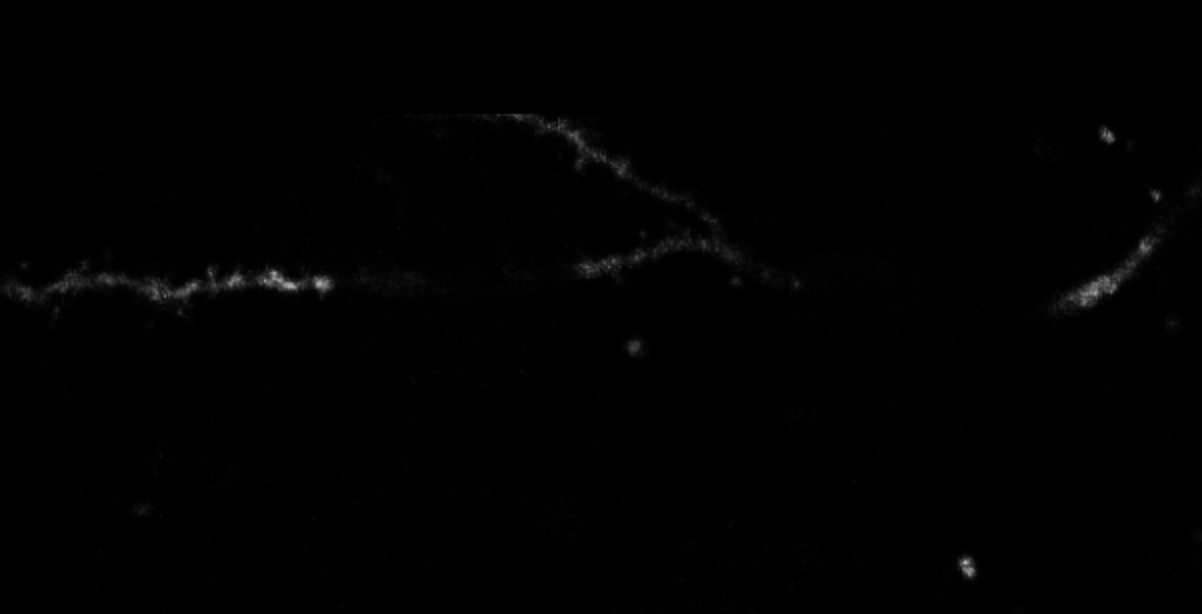
\includegraphics[width=108mm]{images/neu}
\caption{原始神经元图像样例}
\label{neu}
\end{figure}


针对神经元图像的这个特点,可以针对性的传递图片中的神经元组织,忽略掉大面积的黑色背景,这样做会大大降低所需要传递的数据量。但是这样做一方面需要判断图片中的神经组织,增大后端服务器的计算量;另一方面对于一些不同显微镜下的图片神经元在图像中的比例较大,这种优化方式甚至会加大数据传输量。最终采取的解决方案是在后端服务器计算资源空闲的时候对原始图像信息进行处理,对于处理完毕且图像中神经元组织较小的图片只传输神经元组织信息,反之传递原始图像。这样做在绝大多数场景下取得了较高的性能。

\section{平台硬件架构}
在软件编写完成之后,共使用三台计算机作为网络节点,一台计算机部署了神经信息数据库和用户信息数据库,另外两台部署了网络应用服务器用于负载均衡。计算机详细配置如下:

1. 操作系统: Ubuntu 16.04.2 LTS (GNU/Linux 4.4.0-72-generic x86\_64)

2. 中央处理器: Intel(R) Xeon(R) CPU E5-2620 v2 @ 2.10GHz

3. 内存:63149 MB

4. 网卡:Ethernet controller: Broadcom Corporation NetXtreme II BCM57800 1/10 Gigabit Ethernet * 4

5. 硬盘:1.75 TB 机械硬盘

\section{性能优化}

在平台搭建完成后,使用 Gatling\upcite{gatling} 进行了压力测试,数据如图 \ref{origin} 所示。测试中一共模拟了 100 名用户同时访问平台,每位用户模拟进行不同的操作共计 301 次操作,所用用户共计 30100 次操作,平均每秒进行 2508.333 次操作。

\begin{figure}
\centering
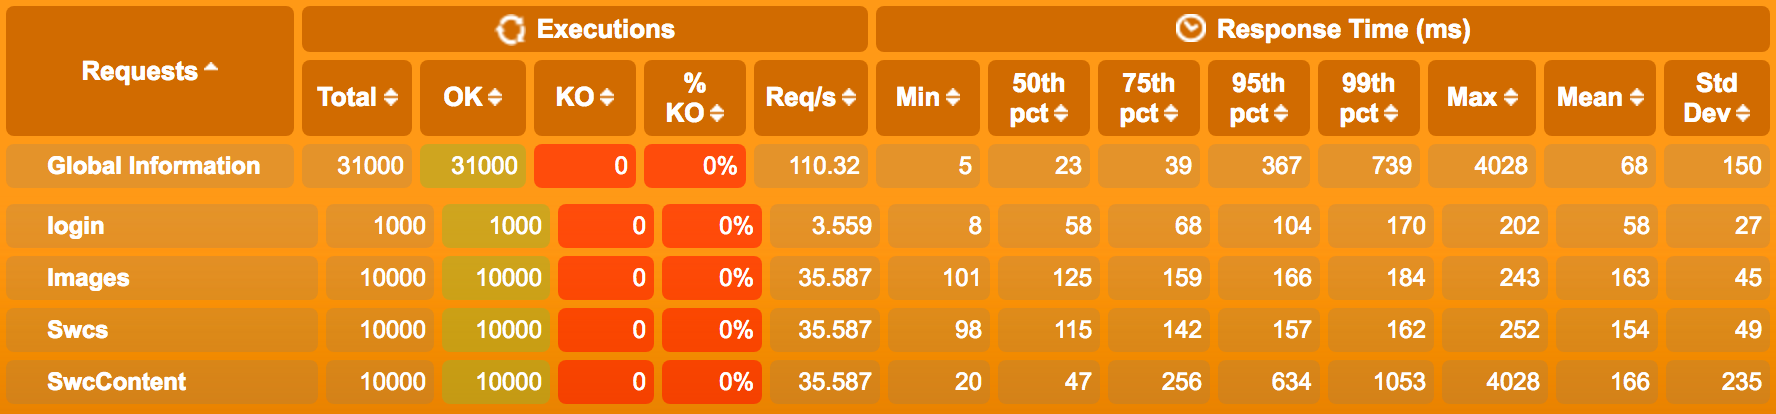
\includegraphics[width=108mm]{images/origin}
\caption{未经过任何优化的性能数据。图中 Login 代表用户登录的请求, Images 代表获取用户原始图像列表相关 API 的响应时间,Swcs 代表用户对神经元结构进行操作的相关 API 的响应时间,SwcContent 代表用户获取结构脑胞体的响应时间。}
\label{origin}
\end{figure}

\subsection{优化获取结构脑胞体的响应时间}
从图 \ref{origin} 中可以看出获取结构脑胞体的响应时间较长,最长响应时间甚至达到了 4028ms,这对于用户来说是可以明显感受到的卡顿,甚至是不可接受的卡顿,这使得需要对获取结构脑胞体的 API 进行优化。考虑到这个 API 需要传输大量的内容,可以认为是传输数据量较大导致的性能问题,可以考虑从减少传输的数据量入手。经过调查相关技术,最终采用两种方式进行优化。第一个方案是采用浏览器端的数据库 indexDB 进行缓存\upcite{network2013indexeddb},将已经获取过的结构脑胞体储存在客户端中,减少了向服务器的请求次数。另一方面,根据 Mogul, Jeffrey C 等人提出的在 HTTP 中使用的编码和压缩方式并结合一些更新的技术对结构脑胞体的数据进行了压缩,是的传输的数据量更小。结合这两点,将获取结构脑胞体的响应时间从 166ms 降低到了 17ms,降低了 89.75\%,具体数值如图 \ref{swccontent},详细的响应时间分布如图 \ref{swcdic} 所示,获取结构脑胞体的响应时间大大降低。

\begin{figure}
\centering

\includegraphics[width=108mm]{images/swccontent}
\caption{经过优化的获取结构脑胞体响应时间,从 166ms 降低到了 17ms,降低了 89.75\%}
\label{swccontent}
\end{figure}

\begin{figure}
\centering
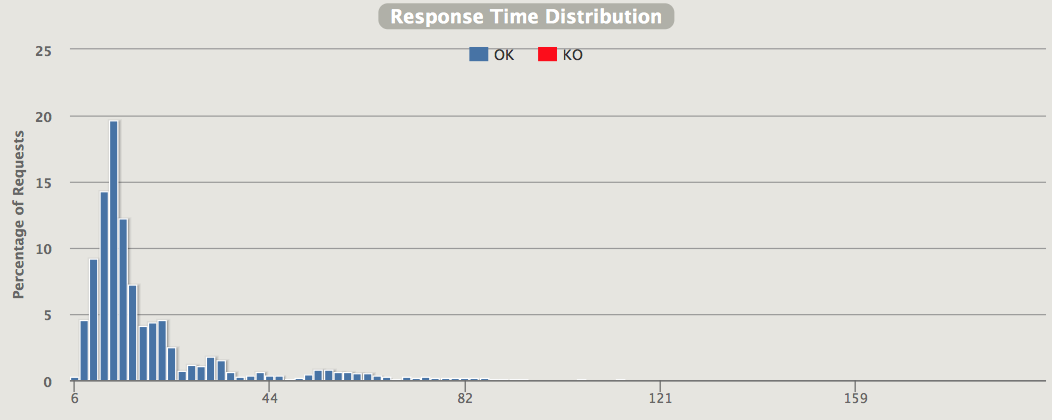
\includegraphics[width=108mm]{images/swcdic}
\caption{经过优化的获取结构脑胞体响应时间分布,绝大多数的响应时间在 6~44 ms 之间,用户感受不到明显的卡顿}
\label{swcdic}
\end{figure}

\subsection{使用 Redis  和负载均衡降低响应时间}
在优化获取结构脑胞体的响应时间的过程中使用了浏览器端的缓存进行优化,这启发我们使用服务器端的缓存来进一步优化。Redis 是一个支持网络、可基于内存亦可持久化的日志型、Key-Value 数据库。由于用户大概率修改编辑最新导入的数据,因此可以将近期的原始图像数据信息缓存在 Redis 之中,减少了请求数据库的次数,提升了整体性能。此外将数据库与网络服务器部署在不同的服务器上,降低了单台服务器的压力,大大提升了每秒响应请求的数量,使之可以支撑更多的用户同时访问。由于网络服务器的处理压力仍然较大,进一步将网络服务器的处理任务分散到两台服务器上,进一步降低了网络服务器的计算压力,优化过后的测试结果如图 \ref{opt} 所示,详细的测试分析在第四章论述。

\begin{figure}
\centering
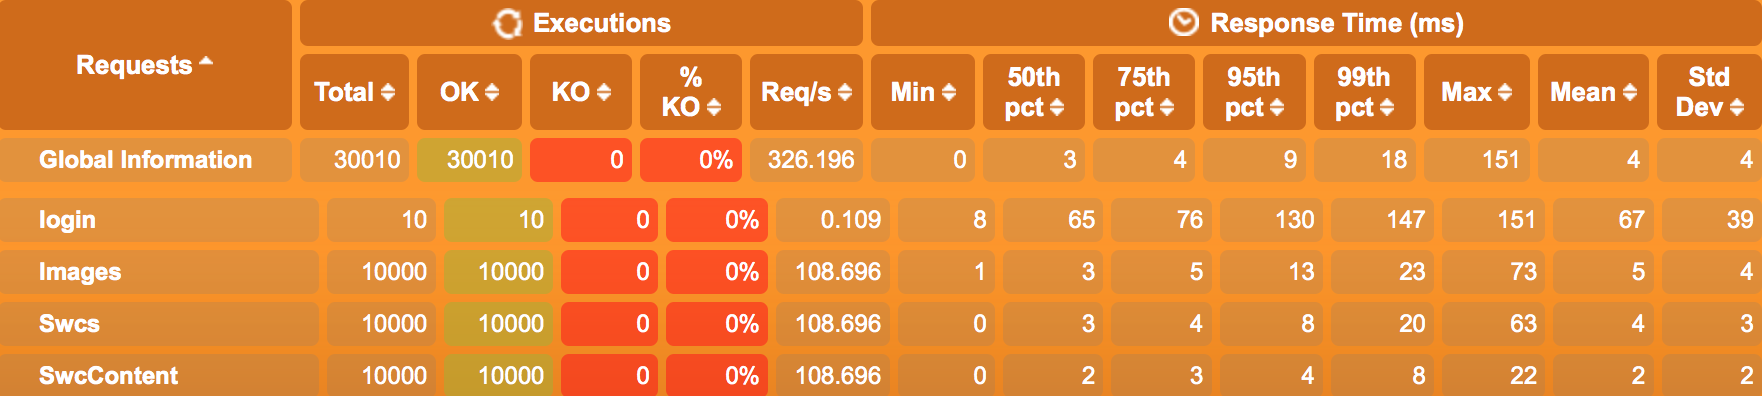
\includegraphics[width=108mm]{images/opt}
\caption{经过优化的整体响应时间报告,图中 Login 代表用户登录的请求, Images 代表获取用户原始图像列表相关 API 的响应时间,Swcs 代表用户对神经元结构进行操作的相关 API 的响应时间,SwcContent 代表用户获取结构脑胞体的响应时间。可以看出绝大多数响应时间都在 100 ms 一下,性能大大提升。}
\label{opt}
\end{figure}